%%%%%%%%%%%%%%%%%%%%%%%%%%%%%%%%%%%%%%%%%%%%%%%%%%%%%%%%%%%%%%%%%%%%%%%%%%%%
%  第16回 解答［17］〜［23］（旧 prob_p126_2.png 〜 prob_p131.png）
%  ※ このファイルは記録用。実体は physics_ch16.tex に流し込み済み。
%%%%%%%%%%%%%%%%%%%%%%%%%%%%%%%%%%%%%%%%%%%%%%%%%%%%%%%%%%%%%%%%%%%%%%%%%%%%

\KaiTitle{第16回　気体の状態変化\MARU{1}}
\setlength{\columnseprule}{0.4pt}
\begin{multicols}{2}
\raggedcolumns

\Rank{A問題}
\MonN{17}{基本事項の確認}\par\nopagebreak
\begin{sisin}
気体がした仕事は$\displaystyle\int P(V)dV$によって計算するが，特に定圧変化（$P(V)=P_0$（一定））の場合に限り，積分の中から$P(V)=P_0$を出して，$P_0\displaystyle\int dV=P_0\cdot\Delta V$と変形できる．
\end{sisin}
\KaiHead
\begin{komon}
\ko{1} $p=$一定のとき，気体の体積変化を$\Delta V$とすれば，気体が外界に対してする仕事$W$は，$W=p\Delta V$と表せるので，
% 誤植訂正（2026-09-02）：原本は「仕事が外界に対してする仕事 W は」と主語が
%   「仕事」になっていたので「気体が…」に改めた．
       \[\begin{aligned}
         W&=(1.0\times 10^5)\cdot(2.0\times 10^{-4})\\
          &=2.0\times 10\U{J}\Ans
       \end{aligned}\]
\ko{2} 熱力学第一法則より$\Delta U=Q+W$が成立するので，
       \[\begin{aligned}
         \Delta U&=4.2\times 10^3+(-2.4\times 10^3)\\
                 &=1.8\times 10^3\U{J}\Ans
       \end{aligned}\]
\end{komon}

\Rank{B問題}
\MonN{18}{気体がする仕事}\par\nopagebreak
\begin{sisin}
気体が外界に対してする仕事$w=$\hskip0pt$\displaystyle\int_{V_{\mathrm{initial}}}^{V_{\mathrm{final}}}P(V)dV$を計算する際，積分区間の下端には最初の状態の体積を，上端には最後の状態の体積を入れる．\underline{最後の状}\hskip0pt\underline{態の体積}\hskip0pt\underline{の方が小}\hskip0pt\underline{さいから}\hskip0pt\underline{といって}\hskip0pt\underline{下端に入}\hskip0pt\underline{れてはな}\hskip0pt\underline{らない！}

$w=\displaystyle\int_{V_{\mathrm{initial}}}^{V_{\mathrm{final}}}P(V)dV$から分かるように，$V_{\mathrm{final}}>V_{\mathrm{initial}}$の場合には気体が外部にする仕事$w$は$p-V$図の曲線と$V$軸とで囲まれる部分の面積を表す．

一方，$V_{\mathrm{final}}<V_{\mathrm{initial}}$の際には$p-V$図の曲線と$V$軸とで囲まれる部分の面積は$\displaystyle\int_{V_{\mathrm{final}}}^{V_{\mathrm{initial}}}P(V)dV$と表される．これは{\gtfamily 気体が外界からされた仕事}を表す．気体が外部にする仕事は，これにマイナスをつけた値である．
\end{sisin}
\KaiHead
\begin{komon}
\ko{1} 次の長方形の面積が求める値である．
       \begin{center}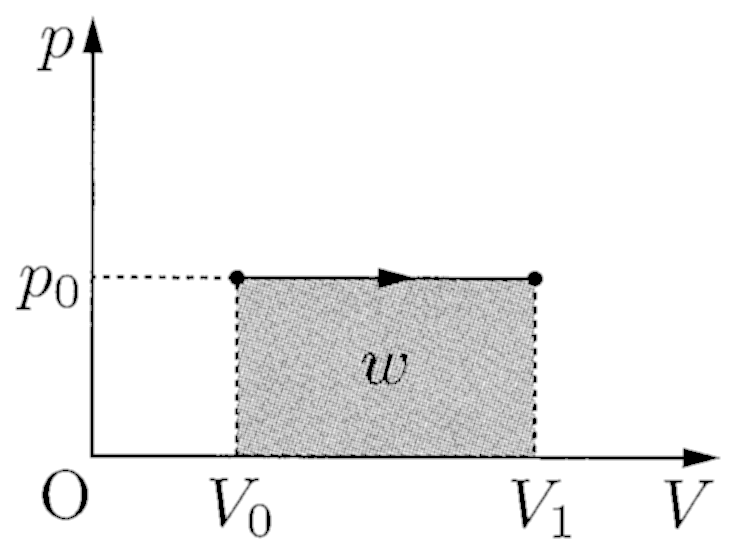
\includegraphics[keepaspectratio,width=46mm]{fig/ch16_a18_1.png}\end{center}
       \[w=p_0(V_1-V_0)\U{J}\Ans\]
\ko{2} 次の台形の面積が求める値である．
       \begin{center}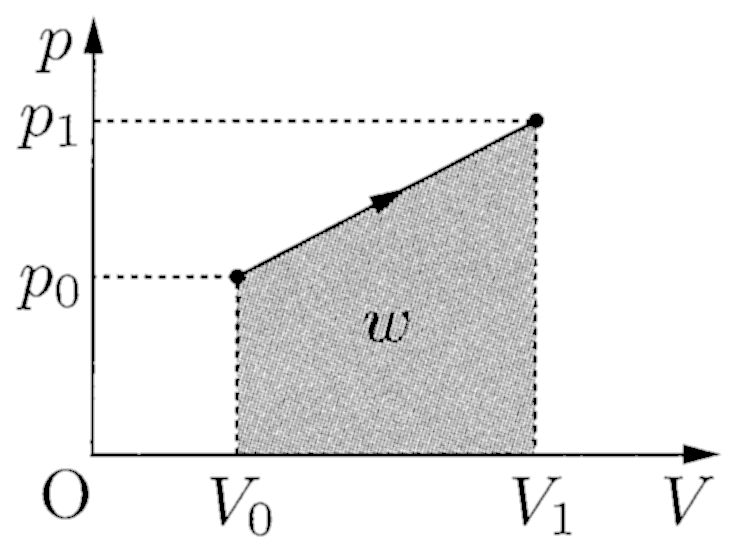
\includegraphics[keepaspectratio,width=46mm]{fig/ch16_a18_2.png}\end{center}
       \[w=\frac{1}{2}(p_0+p_1)(V_1-V_0)\U{J}\Ans\]
\ko{3} 気体の体積変化がないので，
       \[w=0\U{J}\Ans\]
\ko{4} 次の網点部の面積が求める値である．
       \begin{center}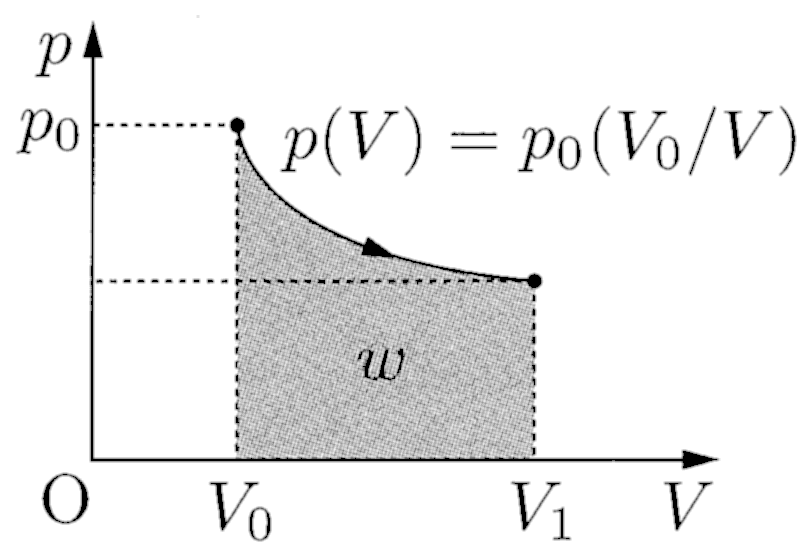
\includegraphics[keepaspectratio,width=48mm]{fig/ch16_a18_4.png}\end{center}
       \[\begin{aligned}
         w&=\int_{V_0}^{V_1}\frac{p_0V_0}{V}dV=p_0V_0\Bigl[\log_e|V|\Bigr]_{V_0}^{V_1}\\
          &=p_0V_0\log_e\frac{V_1}{V_0}\U{J}\Ans
       \end{aligned}\]
\ko{5} 気体が外部からされる仕事を$W$とすると，
       \[W=p_0(V_0-V_1)\U{J}\]
       \begin{center}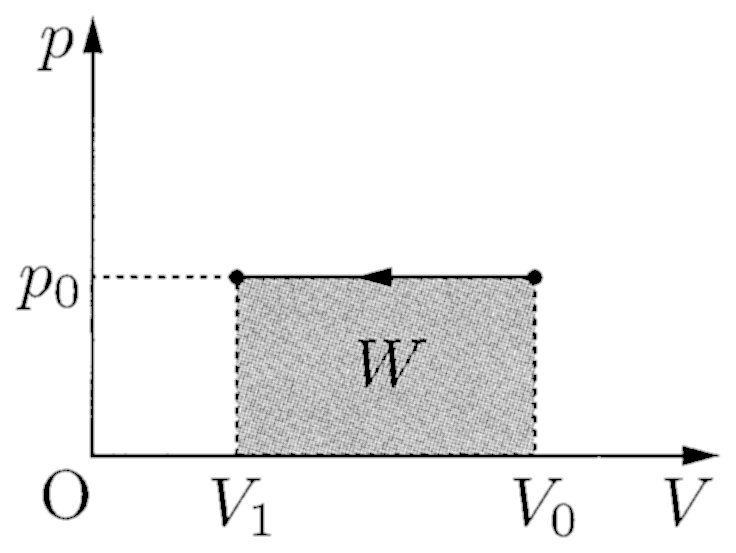
\includegraphics[keepaspectratio,width=46mm]{fig/ch16_a18_5.png}\end{center}
       求めるのは気体が外部にする仕事であるから，
       \[w=-W=-p_0(V_0-V_1)\U{J}\Ans\]
\ko{6} この場合，下の網点部の面積が$W$に等しい．
       \begin{center}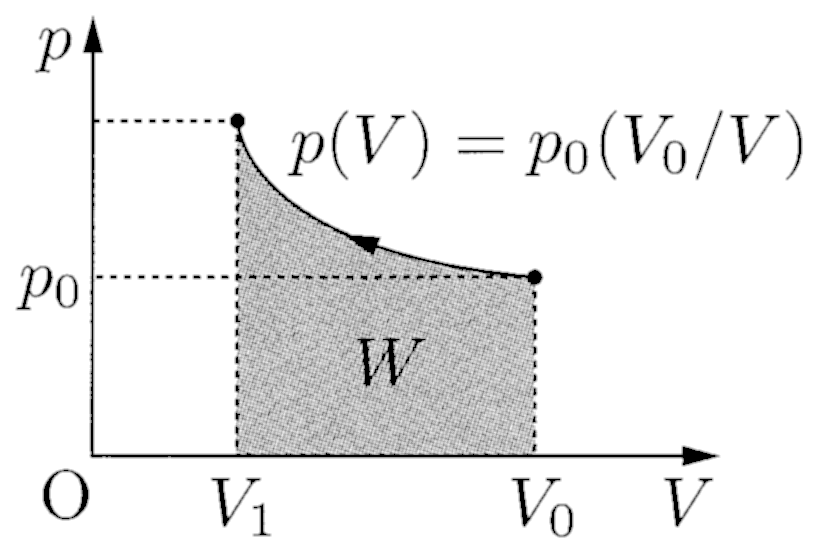
\includegraphics[keepaspectratio,width=48mm]{fig/ch16_a18_6.png}\end{center}
       \[\begin{aligned}
         W&=\int_{V_1}^{V_0}\frac{p_0V_0}{V}dV=p_0V_0\Bigl[\log_e|V|\Bigr]_{V_1}^{V_0}\\
          &=p_0V_0\log_e\frac{V_0}{V_1}\U{J}
       \end{aligned}\]
       求めるのは気体が外部にする仕事であるから，
       \[w=-W=-p_0V_0\log_e\frac{V_0}{V_1}\U{J}\Ans\]
\end{komon}
\begin{bekkai}
各問について$w=\displaystyle\int_{\mathrm{start}}^{\mathrm{end}}P(V)dV$を考えると，
\begin{komon}
\ko{1} $w=\displaystyle\int_{V_0}^{V_1}p_0dV=p_0(V_1-V_0)\U{J}$\Ans
\ko{2} 与えられたグラフより
       \[p(V)=p_0+\frac{p_1-p_0}{V_1-V_0}(V-V_0)\]
       であるから，
       \[\begin{aligned}
         w&=\int_{V_0}^{V_1}\left\{p_0+\frac{p_1-p_0}{V_1-V_0}(V-V_0)\right\}dV\\
          &=\frac{p_0+p_1}{2}(V_1-V_0)\U{J}\Ans
       \end{aligned}\]
% 誤植訂正（2026-09-02）：原本は $\frac{p_1+p_2}{2}$ となっていたが，本問に $p_2$ は
%   登場しない．本解の(2)の答 $\frac12(p_0+p_1)(V_1-V_0)$ と一致する $\frac{p_0+p_1}{2}$ が正しい．
\ko{3} $w=\displaystyle\int_{V_0}^{V_0}P(V)dV=0\U{J}$\Ans
\ko{4} $w=\displaystyle\int_{V_0}^{V_1}\frac{p_0V_0}{V}dV=p_0V_0\Bigl[\log_e|V|\Bigr]_{V_0}^{V_1}$\par
       \hspace*{1zw}$=p_0V_0\log_e\dfrac{V_1}{V_0}\U{J}$\Ans
\ko{5} $w=\displaystyle\int_{V_0}^{V_1}p_0dV=-p_0(V_0-V_1)\U{J}$\Ans
\ko{6} $w=\displaystyle\int_{V_0}^{V_1}\frac{p_0V_0}{V}dV=p_0V_0\Bigl[\log_e|V|\Bigr]_{V_0}^{V_1}$\par
       \hspace*{1zw}$=-p_0V_0\log_e\dfrac{V_0}{V_1}\U{J}$\Ans
\end{komon}
\end{bekkai}
\begin{chuu}
(5), (6)の答えにおいてマイナスを前に出したのは，$V_0>V_1$であるため．このような形にした方が式の正負がはっきり分かる．
\end{chuu}

\MonN{19}{定圧変化}\par\nopagebreak
\begin{sisin}
気体の状態変化の問題では，初状態と終状態の簡単な図を描き，各々の状態について状態方程式を立て，それぞれのときの圧力，体積，温度の三つを整理しておくと分かりやすい．

一般に，気体の状態変化に関して熱力学第一法則を用いる問題は，\MARU{1}気体が外部にする仕事$w=\displaystyle\int_{V_{\mathrm{initial}}}^{V_{\mathrm{final}}}P(V)dV$の計算，\MARU{2} $\Delta U=nC_V\Delta T$の計算，\MARU{3}熱力学第一法則$\Delta U=Q+W$の立式，という流れに沿うものが多い．この\MARU{2}の$\Delta U=nC_V\Delta T$の計算の際に初状態・終状態の温度が必要になるので，各状態での気体の温度はしっかりと押さえること．なお，$\Delta U=nC_V\Delta T$は定積モル比熱$C_V$を用いているが，この式は\underline{定積変化}\hskip0pt\underline{に限らず}\hskip0pt\underline{あらゆる}\hskip0pt\underline{状態変化}\hskip0pt\underline{に関して}\hskip0pt\underline{成立する}式である．

本問の場合，ピストンが自由に動け，かつゆっくり熱を与える（＝ゆっくりと変化させる）とあるので，ピストンの左右の圧力は常につり合っていると考えられる（いずれかの圧力が高ければ，圧力がつり合うような位置にピストンが移動する）．よって，気体の圧力は常に外圧（大気圧）と等しくなっている．

本問では単原子分子の理想気体であるとは書かれていないので，$C_V=\dfrac{3}{2}R$であるとは限らない．勝手に$C_V=\dfrac{3}{2}R$と置かないようにしよう．
\end{sisin}
\KaiHead
\begin{komon}
\ko{1} ピストンが自由に動け，かつゆっくりと変化させているので，この気体の圧力は常に大気圧$p_0\U{Pa}$に等しい．よって，最初の状態について状態方程式を立てると，
       \[p_0\cdot Sl_0=nRT_0\]
       これより，
       \[p_0=\frac{nRT_0}{Sl_0}\U{Pa}\Ans\]
\ko{2} (1)で述べたように，この気体の圧力は常に大気圧$p_0\U{Pa}$に等しい．加熱により体積は$Sl_1\U{m^3}$に増加するので，終状態の気体の状態方程式を立てると，
       \[p_0\cdot Sl_1=nRT_1\]
       これと(1)の状態方程式を組み合わせて解くと，
       \[T_1=\frac{l_1}{l_0}T_0\U{K}\Ans\]
\ko{3} この気体は圧力を常に大気圧$p_0\U{Pa}$に等しく保って状態変化しているので，この状態変化の$p-V$図は次図の通りとなる．
       \begin{center}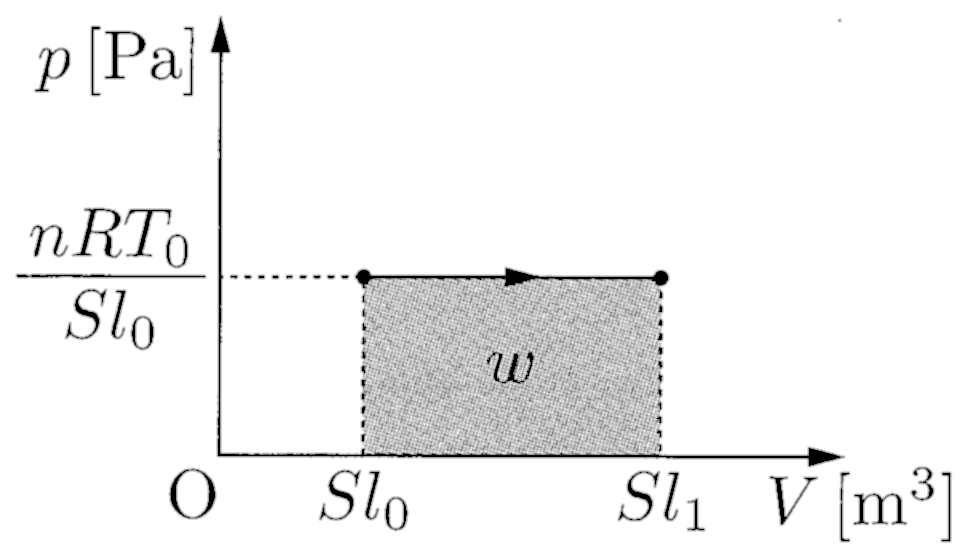
\includegraphics[keepaspectratio,width=58mm]{fig/ch16_a19_pv.png}\end{center}
       \hspace*{\fill}\Ans
\ko{4} この状態変化において気体が外界にした仕事$w\U{J}$は，$Sl_1>Sl_0$ゆえ$p-V$図と$V$軸とで囲まれる部分の面積に相当する．よって(3)の$p-V$図より，
       \[\begin{aligned}
         w&=\frac{nRT_0}{Sl_0}(Sl_1-Sl_0)\\
          &=nRT_0\left(\frac{l_1}{l_0}-1\right)\U{J}\Ans
       \end{aligned}\]
\ko{5} この状態変化における気体の内部エネルギーの増加量を$\Delta U\U{J}$とすると，
       \[\Delta U=nC_V(T_1-T_0)\]
       と書け，これに(2)の値を代入して計算すると，
       \[\Delta U=nC_VT_0\left(\frac{l_1}{l_0}-1\right)\U{J}\]
       ここで熱力学第一法則より，$\Delta U$, $Q$, $w$の間には
       \[\Delta U=Q+(-w)\]
       の関係が成り立つので，(4)および$\Delta U$を代入して，
       \[Q=n(C_V+R)T_0\left(\frac{l_1}{l_0}-1\right)\U{J}\Ans\]
\end{komon}
\begin{bekkai}
この状態変化は定圧変化であるから，この気体の定圧モル比熱を$C_P$とすると，この状態変化での吸熱量は
\[Q=nC_P\Delta T=nC_P(T_1-T_0)\]
と書き下せる．この気体は理想気体ゆえ，$C_V$と$C_P$の間にはマイヤーの関係式
\[C_P=C_V+R\]
が成立する．よって，
\[\begin{aligned}
  Q&=n(C_V+R)(T_1-T_0)\\
   &=n(C_V+R)T_0\left(\frac{l_1}{l_0}-1\right)\U{J}\Ans
\end{aligned}\]
\end{bekkai}
\begin{chuu}
指針において，$\Delta U=nC_V\Delta T$は\underline{定積変化}\hskip0pt\underline{に限らず}\hskip0pt\underline{あらゆる}\hskip0pt\underline{状態変化}\hskip0pt\underline{に関して}\hskip0pt\underline{成立する}式である，と述べたが，逆に\underline{定圧変化}\hskip0pt\underline{の際にし}\hskip0pt\underline{か成立し}\hskip0pt\underline{ない}式は以下の二つである．
\[Q=nC_P\Delta T,\ w=P\cdot\Delta V\]
この2式は定圧変化以外では利用してはならない．
% 誤植訂正（2026-09-02）：原本は「この2式は定積変化以外では利用してはならない」と
%   なっていたが，直前で「定圧変化の際にしか成立しない式」と述べている．
また，\underline{定積でし}\hskip0pt\underline{か}成立しない式は，
\[Q=nC_V\Delta T\]
である．どの式が一般的に利用できて，どれはできないのかをしっかりと区別すること．
% 誤植訂正（2026-09-02）：原本は「どの式は一般的に利用できて」．
\end{chuu}

\MonN{20}{定積変化}\par\nopagebreak
\begin{sisin}
基本的な流れは前問の定圧変化の場合と全く同じで，\MARU{1}気体が外部にする仕事$w=\displaystyle\int_{V_{\mathrm{initial}}}^{V_{\mathrm{final}}}P(V)dV$の計算，\MARU{2} $\Delta U=nC_V\Delta T$の計算，\MARU{3}熱力学第一法則$\Delta U=Q+W$の立式，という流れに従う．

定積変化の特徴は，体積変化がない$\Rightarrow$気体が仕事をしない，ということである．\underline{気体の仕}\hskip0pt\underline{事のやり}\hskip0pt\underline{取りは気}\hskip0pt\underline{体の体積}\hskip0pt\underline{変化に伴}\hskip0pt\underline{って起こ}\hskip0pt\underline{る}ということを押さえておこう．
\end{sisin}
\KaiHead
\begin{komon}
\ko{1} 初状態も終状態も体積は変わらず$Sl_0\U{m^3}$である．初状態・終状態それぞれについて状態方程式を立てると，
       \[\begin{aligned}
         \text{初状態：}&p_0\cdot Sl_0=nRT_0\\
         \text{終状態：}&p_1\cdot Sl_0=nRT_1
       \end{aligned}\]
       これらを解いて，
       \[p_0=\frac{nRT_0}{Sl_0}\U{Pa},\ p_1=\frac{nRT_1}{Sl_0}\U{Pa}\Ans\]
\ko{2} この状態変化は定積変化であるから，$p-V$図上ではグラフは$V$軸に垂直になる．加熱したので$T_1>T_0$であるから，$p_1>p_0$となることに注意すると$p-V$図は次図の通り．
       \begin{center}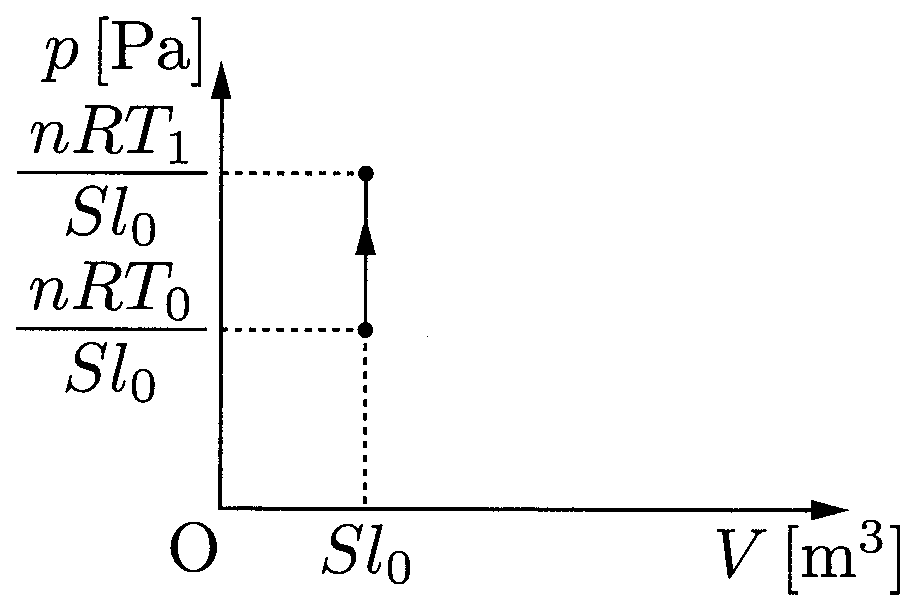
\includegraphics[keepaspectratio,width=52mm]{fig/ch16_a20_pv.png}\end{center}
       \hspace*{\fill}\Ans
\ko{3} この状態変化は定積変化であるから，気体は外界に対して仕事をしない（(2)で，$p-V$曲線と$V$軸が囲む面積が0）．よって，
       \[w=0\U{J}\Ans\]
\ko{4} この状態変化における気体の内部エネルギーの増加量を$\Delta U\U{J}$とすると，
       \[\Delta U=nC_V(T_1-T_0)\ \cdots\mbox{（☆）}\]
       と書ける．\par
       \hspace*{1zw}ここで熱力学第一法則より，$\Delta U$, $Q$, $w$の間には
       \[\Delta U=Q+(-w)\]
       の関係が成り立つので，(3)および$\Delta U$を代入して，
       \[Q=nC_V(T_1-T_0)\U{J}\Ans\]
\end{komon}
\begin{bekkai}
この状態変化は定積変化であるから，定積モル比熱の定義より，
\[\begin{aligned}
  Q&=nC_V\Delta T\\
   &=nC_V(T_1-T_0)\U{J}\Ans
\end{aligned}\]
としてもよい．
\end{bekkai}

\MonN{21}{気体のした仕事}\par\nopagebreak
\begin{sisin}
要するに$w=\displaystyle\int_{V_{\mathrm{initial}}}^{V_{\mathrm{final}}}P(V)dV$を計算すればよいのだから，変化途中の，体積が$V\U{m^3}$になったときの圧力$P(V)$を求め，これを積分すればよい．
\end{sisin}
\KaiHead
\begin{komon}
\ko{1} 膨張前・膨張後の圧力をそれぞれ$P_1$, $P_2\U{Pa}$として気体の状態方程式を立てると，
       \[P_1V_1=nRT_0,\ P_2V_2=nRT_0\]
       である．また，変化途中の体積が$V\U{m^3}$になったときの圧力$P(V)$は，その時の状態方程式
       \[P(V)V=nRT_0\]
       より，
       \[P(V)=\frac{nRT_0}{V}\U{Pa}\]
       である．この式の分子は定数であるから，気体の圧力は体積に反比例して変化する．すなわち，$p-V$図は双曲線となるので，状態変化の$p-V$図は次図．
       \begin{center}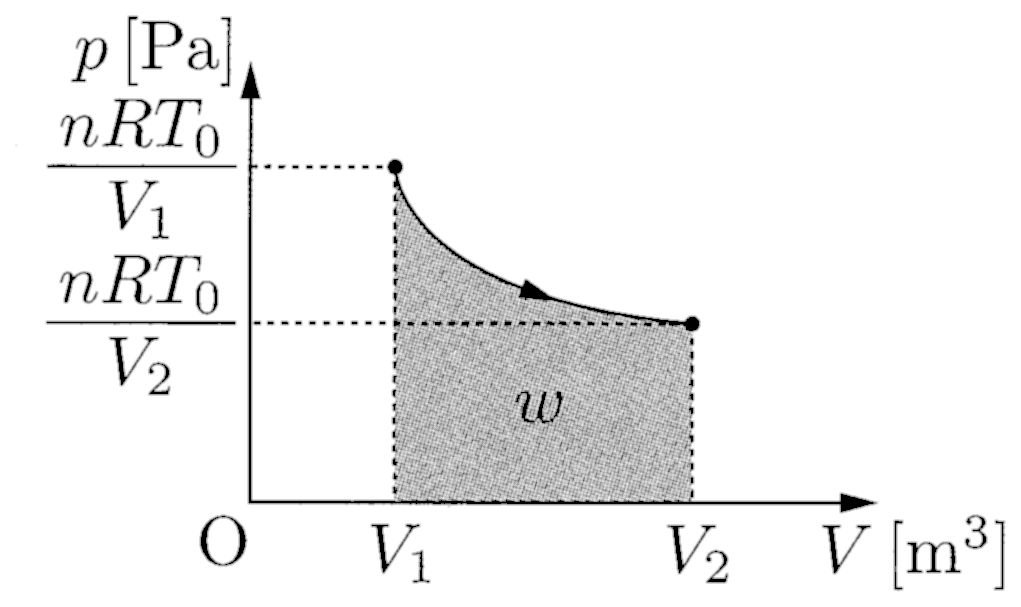
\includegraphics[keepaspectratio,width=60mm]{fig/ch16_a21_pv.png}\end{center}
       \hspace*{\fill}\Ans
\ko{2} 気体は膨張しているので，上の$p-V$図の網点部が気体が外部にした仕事$w$を表す．よって，
       \[\begin{aligned}
         w&=\int_{V_1}^{V_2}\frac{nRT_0}{V}dV=nRT_0\Bigl[\log_e|V|\Bigr]_{V_1}^{V_2}\\
          &=nRT_0\log_e\frac{V_2}{V_1}\U{J}\Ans
       \end{aligned}\]
\end{komon}

\MonN{22}{鉛直シリンダー}\par\nopagebreak
\begin{sisin}
質量$M\U{kg}$のピストンが気体の上に乗っているので，気体の圧力は大気圧$p_0\U{Pa}$と等しくはならない．このような場合には，\underline{ピストン}\hskip0pt\underline{に対して}\hskip0pt\underline{かかる力}\hskip0pt\underline{のつり合}\hskip0pt\underline{いの式を}\hskip0pt\underline{立てて}気体の圧力を求める．

(2)ではピストンがゆっくり動くことから，各瞬間においてピストンに働く力はつりあっていると見なせる．このような変化を準静的変化という．
\end{sisin}
\KaiHead
\begin{komon}
\ko{1} 初状態におけるシリンダー内の圧力を$p\U{Pa}$とする．力の作用図は次図の通りであり，ピストンは静止しているので作用する力がつり合っている．
       \begin{center}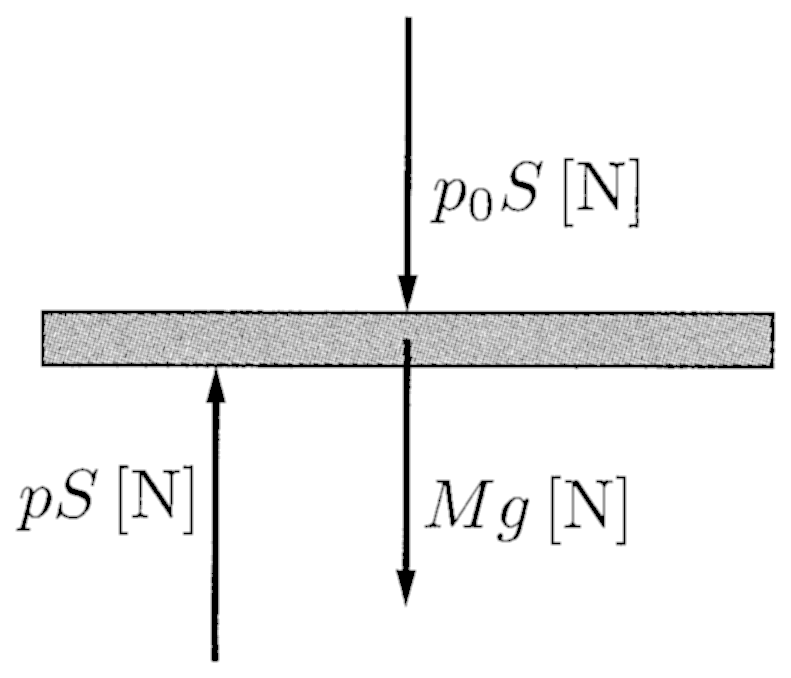
\includegraphics[keepaspectratio,width=44mm]{fig/ch16_a22_f1.png}\end{center}
       この状態の力のつり合いの式は，
       \[pS=p_0S+Mg\]
       ゆえに，
       \[p=p_0+\frac{Mg}{S}\U{Pa}\]
       また，このときの理想気体の状態方程式は，
       \[p(Sl_0)=nRT_0\]
       であるから，これを解いて気体の温度は，
       \[T_0=\frac{(p_0S+Mg)l_0}{nR}\U{K}\Ans\]
\ko{2} ゆっくりと加熱しているからピストンはゆっくりと動いている．よって，このピストンは力のつり合いを保ちつつ動いていると考えられる．変化途中，ピストンに対して作用する力は，(1)と同じく，大気圧による力，気体の圧力による力，重力の三つである．
       \begin{center}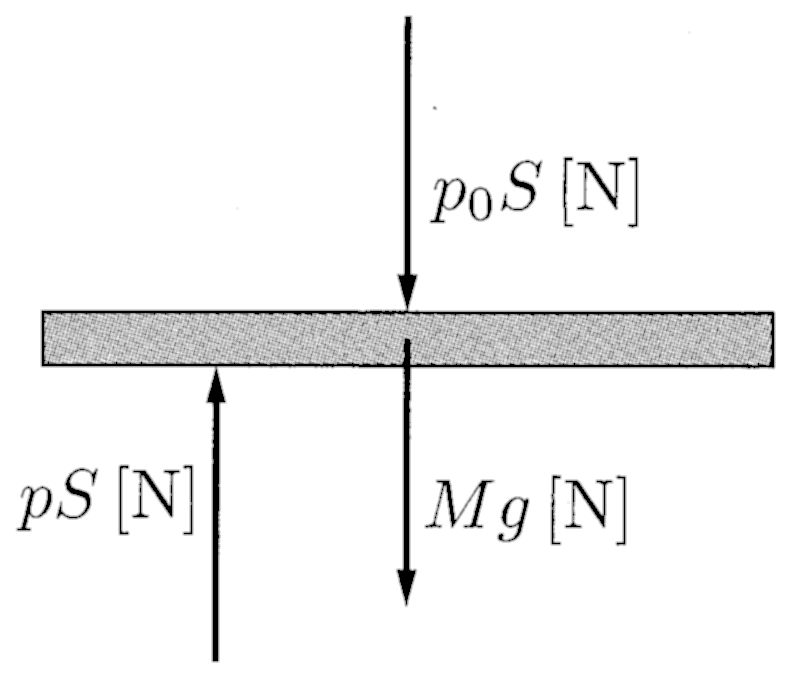
\includegraphics[keepaspectratio,width=44mm]{fig/ch16_a22_f2.png}\end{center}
       よって，変化している最中，ピストンの力のつり合いの式はずっと
       \[pS=p_0S+Mg\]
       のまま変わらないため，内部の気体の圧力は
       \[p=p_0+\frac{Mg}{S}\U{Pa}\]
       のまま変わらない．すなわち，この気体は定圧変化を行う．\par
       \hspace*{1zw}よって，終状態でも気体の圧力は
       \[p=p_0+\frac{Mg}{S}\U{Pa}\]
       であり，終状態での状態方程式
       \[p(Sl_1)=nRT_1\]
       を解いて，
       \[T_1=\frac{(p_0S+Mg)l_1}{nR}\U{K}\Ans\]
\ko{3} 以上より，この気体の状態変化を$p-V$図で表すと次図の通り．
       \begin{center}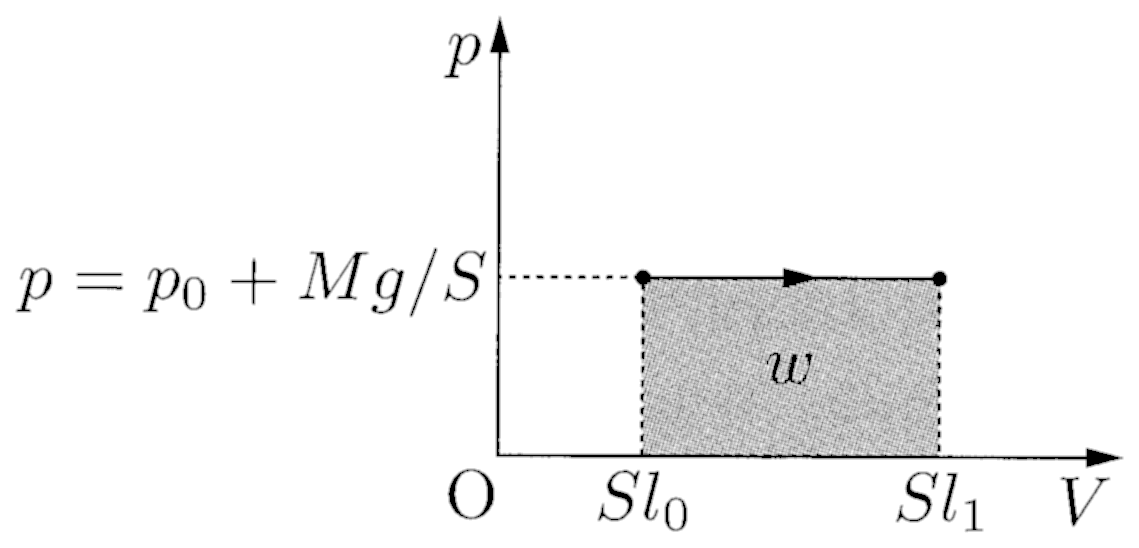
\includegraphics[keepaspectratio,width=66mm]{fig/ch16_a22_pv.png}\end{center}
       よって，この状態変化で気体が外界に対してした仕事$w$は
       \[\begin{aligned}
         w&=\int_{Sl_0}^{Sl_1}pdV=\int_{Sl_0}^{Sl_1}\left(p_0+\frac{Mg}{S}\right)dV\\
          &=(p_0S+Mg)(l_1-l_0)\U{J}\ \cdots\mbox{☆}
       \end{aligned}\]
       また，この変化における気体の内部エネルギーの変化は，
       \[\begin{aligned}
         \Delta U&=nC_V(T_1-T_0)\\
                 &=\frac{C_V(p_0S+Mg)(l_1-l_0)}{R}\U{J}
       \end{aligned}\]
       ここで熱力学第一法則より，
       \[\Delta U=Q+(-w)\]
       の関係が成り立つので，
       \[Q=(p_0S+Mg)(l_1-l_0)\left(1+\frac{C_V}{R}\right)\U{J}\Ans\]
\end{komon}
\begin{bekkai}
この変化は定圧変化であるから，その吸熱量は
\[Q=nC_P(T_1-T_0)\]
である．マイヤーの関係式より$C_P=C_V+R$であるから，
\[Q=n(C_V+R)(T_1-T_0)\]
としても同じ答えを得る．
\end{bekkai}
\begin{bsHosoku}{参考}
☆式にて気体の圧力を積分して$w$を得たが，結果としてその$w$は何に利用されたのかを考えると，
\[w=p_0S(l_1-l_0)+Mg(l_1-l_0)\U{J}\]
と変形すれば，第一項目は大気圧に逆らった仕事，そして第二項目はピストンを持ち上げた位置エネルギー増分であることが分かる．すなわち，$w$は積分を実行しなくても求めることもできる．

$w$が何に利用されるのか直観的に明らかな場合も多いが，より厳密には気体の圧力$p$を与えている式を見れば分かる．$p=p_0+\dfrac{Mg}{S}\U{Pa}$であるのだから，気体が膨張するということは，$p_0$および$\dfrac{Mg}{S}$を押す，ということを意味する．よって，$w$は大気圧に逆らう仕事とピストンを持ち上げる仕事の二つに利用される．本問程度の問題の場合はわざわざこのようなことを考える必要はないが，複雑な問題の場合（バネを含む場合など）はこのことを考えて$w$を求めた方が容易なこともある．
\end{bsHosoku}

\Rank{C問題}
\MonN{23}{定積・定圧変化}\par\nopagebreak
\begin{sisin}
最初の状態ではストッパーに支えられているので，内部の気体がピストンに及ぼす上向きの力の方が，ピストンに対してかかる下向きの力（重力，大気圧による力）よりも小さければピストンは動き出さない．気体を加熱して内圧を上昇させ，上向きの力が下向きの力を上回ったとき初めて動き出す．よって，ピストンが動き出すまでの間は，ピストンに作用する外圧$P_0S$，内圧$PS$，重力$Mg$の三つはつり合ってはいない．このことに注意して考えよ．
\end{sisin}
\KaiHead
\begin{komon}
\ko{1} 初めの状態について，気体の状態方程式を立てると，
       \[p'(Sl_0)=nRT_0\]
       であるから，
       \[p'=\frac{nRT_0}{Sl_0}\U{Pa}\Ans\]
\ko{2} 気体の内圧を$P$とすると，このピストンに対しては図のように力が作用している．
       \begin{center}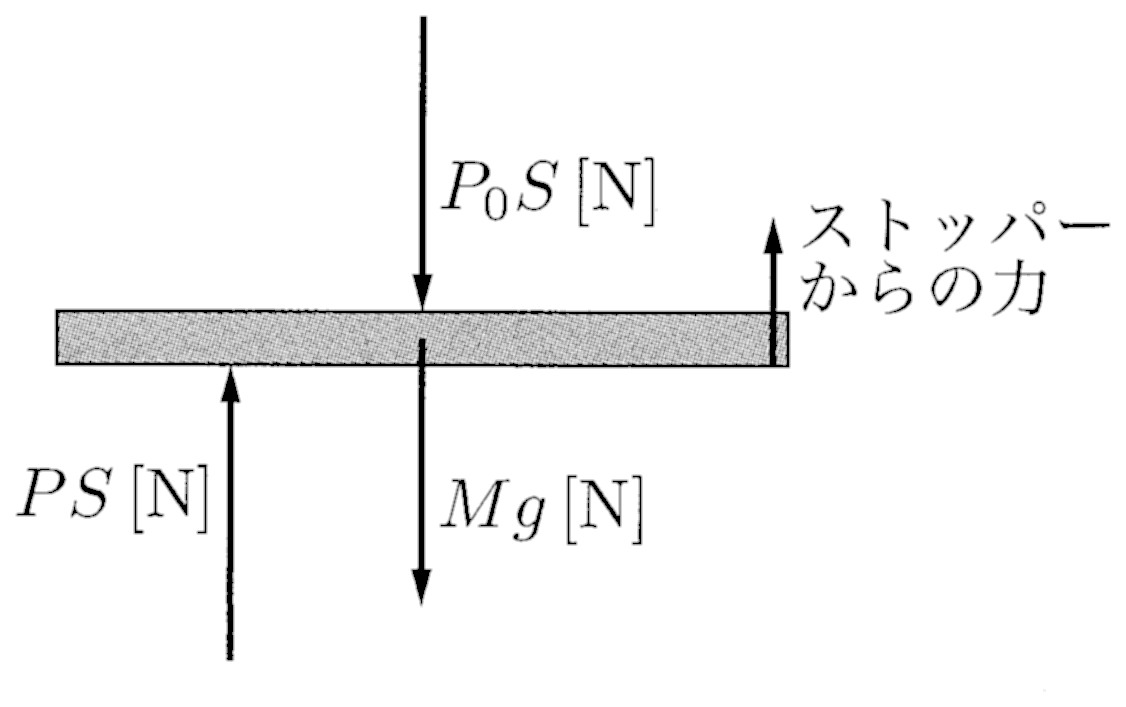
\includegraphics[keepaspectratio,width=66mm]{fig/ch16_a23_f1.png}\end{center}
       ピストンが上昇しはじめるのはストッパーが支える力がなくなったとき，すなわち，
       \[PS\geqq P_0S+Mg\]
       の条件が満たされるようになったときである．ゆえに，このときの気体の圧力$P_1$は
       \[P_1=P_0+\frac{Mg}{S}\U{Pa}\]
       である．この瞬間の気体の体積はまだ$Sl_0\U{m^3}$であることに注意して状態方程式を立てると，
       \[P_1(Sl_0)=nRT_1\]
       であるから，これを解いて，
       \[T_1=\frac{(P_0S+Mg)l_0}{nR}\U{K}\Ans\]
\ko{3} 一旦ピストンが上昇をはじめると，前問と同様，ピストンに作用する力がずっと変わらないため，気体の圧力は
       \[P_1=P_0+\frac{Mg}{S}\U{Pa}\]
       のまま一定となり，定圧変化を続ける．終状態についても気体の圧力はこの$P_1$であるから，終状態についての状態方程式を立てると，
       \[P_1(Sl_1)=nRT_2\]
       であるから，これを解いて，
       \[T_2=\frac{(P_0S+Mg)l_1}{nR}\U{K}\Ans\]
\ko{4} \MARU{1}ピストンが動き始めるまでの間についてと，\MARU{2}ピストンが動き始めてから，とに分けて考える．\par
       \hspace*{1zw}\MARU{1}については気体は定積変化をしているので，この間に気体がした仕事$w_1$は0であり，内部エネルギー変化$\Delta U_1$は，
       \[\Delta U_1=nC_V(T_1-T_0)\]
       である．よってこの間の吸熱量を$Q_1$とすると，熱力学の第一法則より，
       \[\Delta U_1=Q_1+(-w_1)\]
       これより，
       \[Q_1=\Delta U_1+w_1=nC_V(T_1-T_0)\]
       である．また，\MARU{2}については気体は定圧変化をしているので，この間に気体がした仕事$w_2$は
       \[w_2=P_1\cdot\Delta V=P_1\cdot S(l_1-l_0)\]
       であり，内部エネルギー変化$\Delta U_2$は
       \[\Delta U_2=nC_V(T_2-T_1)\]
       である．よってこの間の吸熱量$Q_2$は，熱力学の第一法則より，
       \[\Delta U_2=Q_2+(-w_2)\]
       これより，
       \[\begin{aligned}
         Q_2&=\Delta U_2+w_2\\
            &=nC_V(T_2-T_1)+P_1\cdot S(l_1-l_0)
       \end{aligned}\]
       である．以上より，気体に与えられた総熱量は，
       \[\begin{aligned}
         Q&=Q_1+Q_2\\
          &=nC_V(T_1-T_0)+nC_V(T_2-T_1)\\
          &\hspace*{\fill}+P_1\cdot S(l_1-l_0)\\
          &=\frac{C_V+R}{R}(P_0S+Mg)l_1-nC_VT_0\\
          &\hspace*{\fill}-(P_0S+Mg)l_0\U{J}\Ans
       \end{aligned}\]
\end{komon}
\begin{bekkai}
\MARU{2}についてはマイヤーの関係式$C_P=C_V+R$を用いて考えてもよい．
\[\begin{aligned}
  Q_2&=nC_P(T_2-T_1)\\
     &=n(C_V+R)(T_2-T_1)
\end{aligned}\]
であるから，
\[\begin{aligned}
  Q&=Q_1+Q_2\\
   &=nC_V(T_1-T_0)\\
   &\hspace*{\fill}+n(C_V+R)(T_2-T_1)\\
   &=nC_V(T_2-T_0)+nR(T_2-T_1)\\
   &=n(C_V+R)T_2-nC_VT_0-nRT_1
\end{aligned}\]
と変形して同じ答えを得る．

また，状態変化全体に対して熱力学第一法則を利用するのも手である．\MARU{1}＋\MARU{2}を一つの変化だとみなすと，この間の内部エネルギー変化は
\[\Delta U=nC_V(T_2-T_0)\]
であり，気体が外にした仕事は\MARU{2}のときの
\[w_2=P_1\cdot\Delta V=P_1\cdot S(l_1-l_0)\]
である．これと熱力学第一法則を組み合わせても同じ答えが得られる．
% 誤植訂正（2026-09-02）：原本はこの式を $w_1$ としているが，\MARU{2} の区間の仕事は
%   本解で $w_2$ と置いている（$w_1=0$）．
\end{bekkai}

\end{multicols}
